\documentclass[letterpaper, 10 pt, conference]{sty/ieeeconf}

\IEEEoverridecommandlockouts

\overrideIEEEmargins

\usepackage{graphics}
\usepackage{epsfig}
\usepackage{amsmath}
\usepackage{amssymb}
\usepackage{amsfonts}
\usepackage{txfonts}
\usepackage{tikz}
\usepackage[T1]{fontenc}
\usepackage{cite}
\usepackage[ruled,lined]{algorithm2e}
\usepackage{todonotes}

\usetikzlibrary{shapes,decorations,shadows}
\usetikzlibrary{decorations.pathmorphing}
\usetikzlibrary{decorations.shapes}
\usetikzlibrary{fadings}
\usetikzlibrary{patterns}
\usetikzlibrary{calc}
\usetikzlibrary{decorations.text}
\usetikzlibrary{decorations.footprints}
\usetikzlibrary{decorations.fractals}
\usetikzlibrary{shapes.gates.logic.IEC}
\usetikzlibrary{shapes.gates.logic.US}
\usetikzlibrary{fit,chains}
\usetikzlibrary{positioning}
\usepgflibrary{shapes}
\usetikzlibrary{scopes}
\usetikzlibrary{arrows}
\usetikzlibrary{backgrounds}
\tikzset{latent/.style={circle,fill=white,draw=black,inner sep=1pt, 
minimum size=20pt, font=\fontsize{10}{10}\selectfont},
obs/.style={latent,fill=gray!25},
const/.style={rectangle, inner sep=0pt},
factor/.style={rectangle, fill=gray!25,minimum size=15pt, inner sep=1pt,draw=black},
>={triangle 45}}

\DeclareMathOperator*{\argmax}{arg\,max}
\DeclareMathOperator*{\argmin}{arg\,min}
\DeclareMathOperator{\diag}{diag}
\DeclareMathOperator{\rank}{rank}
\DeclareMathOperator{\card}{card}
\DeclareMathOperator{\atan2}{atan2}

\begin{document}

\title{\LARGE \bf
Self-supervised Calibration for Robotic Systems
}

\author{
\authorblockN{
J\'{e}r\^{o}me Maye,
Paul Furgale,
and Roland Siegwart}
\authorblockA{
Autonomous Systems Lab, ETH Zurich, Switzerland\\
email: \{jerome.maye, paul.furgale, roland.siegwart\}@mavt.ethz.ch}
}

\maketitle

\begin{abstract}In this paper, we address the problem of sensors calibration for mobile robots.
In particular, we are aiming towards an automated system ready to be deployed
for long-term and online operation in the hands of non-experts. To this end, we
augment the classical SLAM formulation with calibration parameters and derive
an MAP estimator that is computed using a Gauss-Newton algorithm. Degenerate
dimensions in sensor data are identified by means of QR decomposition and
automatically discarded from the optimization via a truncated method, such that
only observable parts are exploited. Finally, incoming sensor data is processed
in batch and selected using an information theoretic measure. Through an
extensive set of simulated and real-world experiments, we demonstrate that our
method outperforms state-of-the-art algorithms in terms of applicability,
accuracy, and speed.

\end{abstract}

\section{Introduction\label{intro}}
\cite{bishop06pattern}

The remainder of the paper is structured as follows.


\section{Related Work\label{sec:rel}}


The problem of sensor calibration has been a recurring one in the history of
robotics and computer vision. Thereby, it has been addressed using a
variety of sensor setups and algorithms. A calibration process may involve
recovering \emph{intrisic}, e.g. focal length for a camera, and \emph{extrinsic}
parameters, i.e. the rigid transformation between the sensor's coordinate system
and a reference coordinate system. For the former, one could devise a naive
approach where the parameters are accurately determined during the manufacturing
process. Similarly, the transformation could be retrieved by means of
some measuring instrument. However, the disadvantages of such purely
engineered methods are manifold. Apart from their impracticality, it can be
nearly impossible to reach a satisfying accuracy and thus hinder the proper use
of the sensor in a robotic system. Furthermore, external factors such as
temperature variations or mechanical shocks may seriously bias a factory
calibration. Therefore, much efforts have been dedicated over the years to
develop algorithms for calibration of systems in the field.

The use of a known calibration pattern such as a checkerboard coupled with
nonlinear regression has become the most popular method in computer vision
during the last decade. It has been deployed both for intrinsic camera
calibration~\cite{sturm99plane} and extrinsic calibration
between heterogeneous sensors~\cite{zhang04extrinsic}. While being relatively
efficient, this procedure still requires expert knowledge to reach a good level
of accuracy. It can also be quite inconvenient on a mobile platform requiring
frequent recalibration.

In an effort to automate the process in the context of mobile robotics, several
authors have included the calibration problem in a state-space estimation
framework, either with filtering~\cite{martinelli06automatic} or
smoothing~\cite{kuemmerle11simultaneous} techniques. Filtering techniques based
on the Kalman filter are appealing due to their inherently online nature.
However, in case of nonlinear systems, smoothing techniques based on iterative
optimization are usually superior in terms of accuracy. While building on this
latter method, our approach attempts to reduce its computational load and copes
with degenerate cases.

More recently, Brookshire and Teller~\cite{brookshire12extrinsic} have carried
out a formal observability analysis in order to identify degenerate paths of
the calibration run. In contrast to the method presented in this paper, their
approach still expects that the robot travels along non-degenerate paths.

A last class of methods relies on an energy function to be minimized. For
instance, Levinson and Thrun~\cite{levinson10unsupervised} have defined an
energy function based on surfaces and Sheehan \emph{et al.}~\cite{sheehan12self}
on an information theoretic quantity measuring point cloud quality.

To the best of the authors' knowledge, little research has been devoted to
efficiently deal with degenerate cases frequently occurring during calibration.
The majority of the authors indeed assumes that their optimization routine runs
on well-behaved data. As demonstrated in the next sections, this can be a
critical point in real-world scenarios. In contrast, our approach does not
require any of these assumptions and is suitable for online, autonomous, and
long-term operations on various platforms and sensors.


\section{Model\label{sec:model}}
\subsection{Problem Formulation\label{subsec:prob}}

In the following, we outline our problem in a probabilistic manner, closely
following the discrete-time Simultaneous Localization and Mapping (SLAM)
formulation~\cite{durrantwhyte06simultaneous}. For the sake of clarity, we
consider here a robot with a single sensor observing a known number of landmarks
at each timestep. Furthermore, we assume the correspondences between sensor's
measurements and landmarks are known. The relaxation of these assumptions goes
beyond the scope of this paper.

Let
$\mathcal{X}=\{\mathbf{x}_{0:K}\}$ be a set of \emph{latent} random variables
(LRV) representing robot states up to timestep $K$,
$\mathcal{U}=\{\mathbf{u}_{1:K}\}$ a set of \emph{observable} random variables
(ORV) representing measured control inputs, $\mathcal{L}=\{\mathbf{l}_{1:N}\}$ a
set of LRV representing $N$ landmarks' positions,
$\mathcal{Z}=\{\mathbf{z}_{1_{1:N}:K_{1:N}}\}$ a set of ORV representing $KxN$
landmarks' measurements, and $\boldsymbol{\Theta}$ a LRV representing the
calibration parameters of the robot's sensor. The goal of the calibration
procedure is to compute the posterior marginal distribution of
$\boldsymbol{\Theta}$ given all the measurements up to timestep $K$

\begin{equation}\label{eqn:post_calib}
  \begin{aligned}
  p(\boldsymbol{\Theta}\mid\mathcal{U},\mathcal{Z}) &=
    \int_{\mathcal{X}, \mathcal{L}}p(\boldsymbol{\Theta}, \mathcal{X},
    \mathcal{L} \mid\mathcal{U},\mathcal{Z}).
  \end{aligned}
\end{equation}

The full joint posterior on the left-hand side of \eqref{eqn:post_calib} may
further be factorized into

\begin{equation}\label{eqn:post_joint_factorized}
  \begin{aligned}
  p(\boldsymbol{\Theta}, \mathcal{X},
    \mathcal{L} \mid\mathcal{U},\mathcal{Z}) &\propto\\
    p(\boldsymbol{\Theta}, \mathbf{x}_0,\mathcal{L})
    \prod_{k=1}^K p(\mathbf{x}_k\mid\mathbf{x}_{k - 1},\mathbf{u}_k)
    \prod_{k=1}^K\prod_{i=1}^N p(\mathbf{z}_{k_i}\mid\mathbf{x}_k,
    \mathbf{l}_i,\boldsymbol{\Theta}).
  \end{aligned}
\end{equation}

We may approximate \eqref{eqn:post_joint_factorized} with a normal distribution
whose moments $\boldsymbol{\mu}_{\boldsymbol{\Theta}\mathcal{X}\mathcal{L}}$ and
$\boldsymbol{\Sigma}_{\boldsymbol{\Theta}\mathcal{X}\mathcal{L}}$ have to be
estimated. To this end, we first derive a Maximum a Posteriori (MAP) estimator
for the mean

\begin{equation}\label{eqn:map_estimator}
  \begin{aligned}
  \hat{\boldsymbol{\mu}}_{\boldsymbol{\Theta}\mathcal{X}\mathcal{L}} &=
    \argmax_{\boldsymbol{\Theta},\mathcal{X},\mathcal{L}}
    p(\boldsymbol{\Theta}, \mathcal{X},\mathcal{L} \mid\mathcal{U},\mathcal{Z})
    \\
    &= \argmin_{\boldsymbol{\Theta},\mathcal{X},\mathcal{L}}-\log
    p(\boldsymbol{\Theta}, \mathcal{X},\mathcal{L} \mid\mathcal{U},\mathcal{Z}).
  \end{aligned}
\end{equation}

We further refine our problem by defining a \emph{motion} and \emph{observation}
model

\begin{equation}\label{eqn:process_model}
  \begin{aligned}
  \mathbf{x}_k &= \mathbf{h}(\mathbf{x}_{k-1}, \mathbf{u}_k, \mathbf{w}_k)\\
  \mathbf{z}_{k_i} &= \mathbf{g}(\mathbf{x}_{k}, \mathbf{l}_i, \mathbf{n}_k),
  \end{aligned}
\end{equation}

where

\begin{equation}\label{eqn:noise_model}
  \begin{aligned}
  \mathbf{w}_k \sim \mathcal{N}(\mathbf{0},\mathbf{Q}_k)\\
  \mathbf{n}_k \sim \mathcal{N}(\mathbf{0},\mathbf{R}_k)
  \end{aligned}
\end{equation}

are normally distributed process and observation noise variables,
$\mathbf{Q}_k$ and $\mathbf{R}_k$ being known covariance matrices. The functions
$\mathbf{h}(\cdot)$ and $\mathbf{g}(\cdot)$ might be non-linear in their
parameters.

\subsection{Least Squares Solution}
In case of linear motion and observation models, there exists a closed-form
solution to \eqref{eqn:map_estimator} based on the \emph{least squares} method
due to the normally distributed noise variables. In the other case, one can
resort to non-linear least squares methods that iteratively solve a linearized
version of the problem. In the following, we employ the \emph{Gauss-Newton}
algorithm for this purpose. \textit{Quick derivation of the algorithm to end up with}

\begin{equation}\label{eqn:dx_update}
  \begin{aligned}
  (\mathbf{H}^T\mathbf{T}^{-1}\mathbf{H})\delta\mathbf{x} &=
    -\mathbf{H}^T\mathbf{T}^{-1}\mathbf{e}(\mathbf{x}).
  \end{aligned}
\end{equation}

At convergence of the algorithm, the quantity
$\mathbf{H}^T\mathbf{T}^{-1}\mathbf{H}$ is the \emph{Fisher Information Matrix}
(FIM) and the precision matrix
$\hat{\boldsymbol{\Sigma}}_{\boldsymbol{\Theta}\mathcal{X}\mathcal{L}}^{-1}$ of
our estimate
$\hat{\boldsymbol{\mu}}_{\boldsymbol{\Theta}\mathcal{X}\mathcal{L}}$.

If we let $\mathbf{T}^{-1}=\mathbf{L}^T\mathbf{L}$ be the Cholesky
decomposition of the precision matrix, \eqref{eqn:dx_update} can be rewritten as

\begin{equation}\label{eqn:dx_update_normal}
  \begin{aligned}
  (\mathbf{L}\mathbf{H})^T(\mathbf{L}\mathbf{H})\delta\mathbf{x} &= 
    -(\mathbf{L}\mathbf{H})^T\mathbf{e}(\mathbf{x}),
  \end{aligned}
\end{equation}

which we can recognize as the \emph{normal equations} of the linear system

\begin{equation}\label{eqn:dx_update_standard}
  \begin{aligned}
  (\mathbf{L}\mathbf{H})\delta\mathbf{x} &= -\mathbf{e}(\mathbf{x}).
  \end{aligned}
\end{equation}

Thus, instead of directly solving \eqref{eqn:dx_update} which requires a
significant amount of computation and introduces numerical errors, we can take
advantage of matrix decompositions.

Let $\mathbf{L}\mathbf{H}$ be of size $m*n$ with the following thin
Singular Value Decompostion (\emph{SVD}) decomposition

\begin{equation}\label{eqn:svd_decomposition}
  \begin{aligned}
  \mathbf{L}\mathbf{H} &= \mathbf{U}_n\mathbf{S}_n\mathbf{V}_n^T,
  \end{aligned}
\end{equation}

where $\mathbf{U}_n$ is $m*n$, $\mathbf{S}_n=\diag(\sigma_1, \cdots, \sigma_n)$,
$\mathbf{V}_n$ is $n*n$, and $\sigma_i$ are the singular values of
$\mathbf{L}\mathbf{H}$.

From \eqref{eqn:svd_decomposition} and using the orthogonal property of
$\mathbf{U}_n$ and $\mathbf{V}_n$, we can solve \eqref{eqn:dx_update} as

\begin{equation}\label{eqn:dx_svd_solve}
  \begin{aligned}
  \delta\mathbf{x} &= -\mathbf{V}_n\mathbf{S}_n^{-1}\mathbf{U}_n^T
    \mathbf{e}(\mathbf{x}).
  \end{aligned}
\end{equation}

Although useful for illustrating the concepts of our approach, the SVD
decomposition can be computationally demanding for large matrices. In practice,
we therefore use the thin \emph{QR} decomposition of $\mathbf{L}\mathbf{H}$

\begin{equation}\label{eqn:qr_decomposition}
  \begin{aligned}
  \mathbf{L}\mathbf{H}\boldsymbol{\Pi} &= \mathbf{Q}_n\mathbf{R}_n,
  \end{aligned}
\end{equation}

where $\boldsymbol{\Pi}$ is a permutation matrix, $\mathbf{Q}_n$ is $m*n$, and
$\mathbf{R}_n$ is $n*n$.

From \eqref{eqn:qr_decomposition} and using orthogonal property of
$\mathbf{Q}_n$, \eqref{eqn:dx_update} can be expressed as

\begin{equation}\label{eqn:dx_qr_solve}
  \begin{aligned}
  \mathbf{R}_n\boldsymbol{\Pi}^{T}\delta\mathbf{x} &=
    -\mathbf{Q}_n^T \mathbf{e}(\mathbf{x}),
  \end{aligned}
\end{equation}

which, due the upper triangular form of $\mathbf{R}_n$ can be easily solved by
\emph{back substitution}.

\subsection{Truncated QR Solution}

\subsection{Selecting Informative Measurements}



\section{Experiments\label{sec:exp}}
In order to evaluate and validate the approach proposed in this paper, we have
conducted experiments on simulated and real-world data. We shall first start
with the description of the experimental conditions and then demonstrate the
performance of our algorithm, along with some comparisons against existing
methods.

\subsection{Experimental Setup}

Our method has been fully implemented in MATLAB and we have used the
SuiteSparseQR~\cite{davis11algorithm} package for performing sparse matrices
operations.

Although our eventual goal is full, self-supervised calibration for an
autonomous vehicle system with multiple heterogeneous sensors, the
experiments in this paper are based on a realistic, but somewhat
simplified robotic system. This allows us to precisely control the
observability properties in simulation and test the behavior of our
algorithm.

Fig.~\ref{fig:exp_setup} depicts our experimental setup. The platform
is a differential drive mobile robot equipped with a range sensor
delivering range and bearing measurements. The calibration parameters
of the range sensor consist in the transformation of its coordinate
system to the robot's coordinate system. The platform is further
endowed with wheel odometers outputting translational and rotational
speeds. While navigating on the plane, the robot observes a known
number of landmarks through its range sensor. Both the range sensor 
and the odometry produce data at 10 Hz.

\begin{figure}[t]
\centering
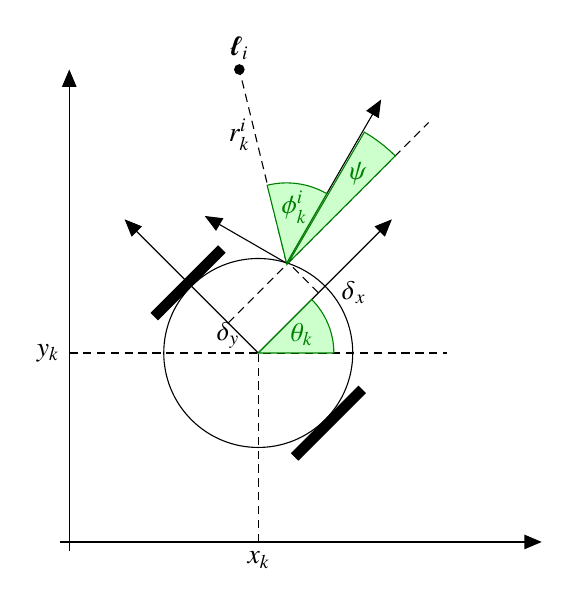
\begin{tikzpicture}[scale = 1.2]
  % styles
\tikzstyle{axes}=[]
\tikzstyle{robot} = []
\tikzstyle{wheels} = [fill]
\tikzstyle{landmark} = [fill]
\tikzstyle{lrf measurement} = [densely dashed]
\colorlet{anglecolor}{green!50!black}

% world axes
\begin{scope}[style = axes]
  \draw[->] (-0.1, 0) -- (5, 0);
  \draw[->] (0, -0.1) -- (0, 5);
\end{scope}

% robot base
\begin{scope}[style = robot, xshift = 2cm, yshift = 2cm, rotate = 45]
  \draw (0, 0) circle (1);
  \draw[wheels] (-0.5, 1) rectangle (0.5, 1.1);
  \draw[wheels] (-0.5, -1) rectangle (0.5, -1.1);
\end{scope}

% robot axes
\begin{scope}[style = axes, xshift = 2cm, yshift = 2cm, rotate = 45]
  \draw[->] (0, 0) -- (2, 0);
  \draw[->] (0, 0) -- (0, 2);
\end{scope}

% lrf axes
\begin{scope}[style = axes, xshift = 2.3cm, yshift = 2.95cm, rotate = 60]
  \draw[->] (0, 0) -- (2, 0);
  \draw[->] (0, 0) -- (0, 1);
\end{scope}

% landmark
\begin{scope}[style = landmark, xshift = 1.8cm, yshift = 5cm, rotate = 0]
  \draw[landmark] (0, 0) circle (0.05) node[above] {$\boldsymbol{\ell}_i$};
\end{scope}

% lrf range measurement
\begin{scope}[style = lrf measurement]
  \draw (2.3, 2.95) -- (1.8, 5) node[left = 0.1cm, below = 0.5cm] {$r^i_k$};
\end{scope}

% lrf bearing measurement
\begin{scope}[xshift = 2.3cm, yshift = 2.95cm, rotate = 60]
  \filldraw[fill = green!20, draw = anglecolor] (0, 0) -- (8.5mm, 0) arc
    (0:44:8.5mm) -- cycle;
  \draw (22:6mm) node[anglecolor] {$\phi^i_k$};
\end{scope}

% robot pose
\begin{scope}
  \draw[densely dashed] (2, 0) node[below] {$x_k$} -- (2, 2);
  \draw[densely dashed] (0, 2) node[left] {$y_k$} -- (4, 2);
  \filldraw[fill = green!20, draw = anglecolor] (2, 2) -- (2.8, 2) arc
    (0:45:0.8) -- cycle;
  \draw[xshift = 2cm, yshift = 2cm] (22.5:0.5) node[anglecolor] {$\theta_k$};
\end{scope}

% lrf pose
\begin{scope} [xshift = 2cm, yshift = 2cm, rotate = 45]
  \draw[densely dashed] (0.9, 0) node[below = -1pt, right = 5pt] {$\delta_x$}
    -- (0.9, 0.45);
  \draw[densely dashed] (0, 0.45) node[left = 3pt, below = -3.8pt] {$\delta_y$}
    -- (3, 0.45);
  \filldraw[fill = green!20, draw = anglecolor] (0.9, 0.45) -- (2.5, 0.45) arc
    (0:14.8:1.6) -- cycle;
  \draw[xshift = 0.9cm, yshift = 0.45cm] (7:1.2) node[anglecolor] {$\psi$};
\end{scope}

\end{tikzpicture}
\caption{Experimental setup. A 2D robot moving in a plane and observing
  landmarks with a range sensor providing range and bearing angle measurements.
  The calibration process needs to find the 2D transformation between the
  robot's coordinate system and the sensor's coordinate system.}
\label{fig:exp_setup}
\end{figure}

More formally, we adopt the following motion and observation models

\begin{equation}\label{eqn:exp_model}
  \begin{aligned}
  \underbrace {
  \begin{pmatrix}
  x_k\\
  y_k\\
  \theta_k
  \end{pmatrix}}_{\mathbf{x}_k}&=
  \underbrace{
  \begin{pmatrix}
  x_{k-1}\\
  y_{k-1}\\
  \theta_{k-1}
  \end{pmatrix} + T
  \begin{pmatrix}
  \cos\theta_{k-1}&0\\
  \sin\theta_{k-1}&0\\
  0&1
  \end{pmatrix}
  \left(\begin{pmatrix}
  v_k\\
  w_k
  \end{pmatrix}
  + \mathbf{w}_k\right)
  }_{\mathbf{h}(\mathbf{x}_{k-1}, \mathbf{u}_k, \mathbf{w}_k)}\\
  a &= x_i - x_k - \delta_x\cos\theta_k + \delta_y\sin\theta_k\\
  b &= y_i - y_k - \delta_x\sin\theta_k - \delta_y\cos\theta_k\\
  \underbrace {
  \begin{pmatrix}
  r_k^i\\
  \phi_k^i
  \end{pmatrix} }_{\mathbf{z}_{k_i}}&=
  \underbrace {
  \begin{pmatrix}
  \sqrt{a^2 + b^2}\\
  \atan2(b, a) - \theta_k - \psi
  \end{pmatrix}
  + \mathbf{n}_k}_{\mathbf{g}(\mathbf{x}_{k}, \boldsymbol{\ell}_i,
    \boldsymbol{\Theta}, \mathbf{n}_k)},
  \end{aligned}
\end{equation}

\noindent where $\mathbf{x}_k=[x_k\;y_k\;\theta_k]^T$ denotes the robot pose at
timestep $k$, $T$ the sampling period, $\mathbf{u}_k=[v_k\;w_k]^T$ the measured
translational and rotational speeds, $\mathbf{z}_{k_i}=[r_k^i\;\phi_k^i]^T$ the
range and bearing observation of landmark $i$ with pose
$\boldsymbol{\ell}_i=[x_i\;y_i]^T$, $\mathbf{w}_k\sim\mathcal{N}(\mathbf{0},
\mathbf{W}_k)$ with $\mathbf{W}_k=\diag(\sigma^2_v,\sigma^2_w)$,
$\mathbf{n}_k\sim\mathcal{N}(\mathbf{0}, \mathbf{N}_k)$ with
$\mathbf{N}_k=\diag(\sigma^2_r,\sigma^2_\phi)$, and
$\mathbf{\Theta}=[\delta_x\;\delta_y\;\psi]^T$ the range sensor's calibration
parameters.

Throughout our experiments, we have used a non-informative prior
$p(\boldsymbol{\Theta}, \mathbf{x}_0, \mathcal{L})$, i.e., a uniform
distribution. The use of priors is still subject to controversial
discussions~\cite{gelman08objections} between Bayesian and non-Bayesian
statisticians. Here, we argue that everything should come from the data itself
and not from some subjective prior information that could bias the inference.

Our algorithm requires only 3 free parameters, namely the rank threshold
$\epsilon$, the batch size $k$, and the MI threshold $\lambda$. Optimally, $k$
should be inferred from the dynamics of the system. While a large $k$
induces storage of uninformative measurements, a small $k$ leads to useless
runs of optimization and makes it difficult to discover informative sequences 
of measurements. In this
setup, we have used a batch size of $k=100$ (ten seconds of data). Concerning
the MI threshold, a small $\lambda$ will keep most of the measurements and a
large $\lambda$ will ignore them all. We have set this value to
$\lambda=0.5$ [bits] in our experiments. The $\epsilon$ parameter shall be
discussed below.

\subsection{Simulated Data}

In our simulation environment, we can generate various paths for the robot,
along with corresponding sensor measurements, and thus analyze the behavior of
multiple algorithms, especially in degenerate cases. We have created an
environment with $N=17$ landmarks uniformly distributed on a $20m\times 20m$
grid. We have set the noise parameters empirically to
$\sigma^2_v=4.4\times 10^{-3}$, $\sigma^2_w=8.2\times 10^{-2}$,
$\sigma^2_r=9.0036\times 10^{-4}$, and $\sigma^2_\phi=6.7143\times 10^{-4}$. The
calibration parameters are fixed at $\delta_x=0.219$ [m], $\delta_y=0.1$ [m],
and $\psi=\pi/4$ [rad].

In a first effort, we want to support the claims of Sec.~\ref{sec:tsvd} with
a representative example. We simulated the robot driving along a straight
path as shown in Fig.~\ref{fig:straight-path}. Intuitively, the problem is
structurally unobservable. Indeed, it has 5 unobservable parameters, 3
corresponding to the global pose of the map and trajectory (as no global
measurements or prior are included) and 2 for the calibration offset variables
$\delta_x$ and $\delta_y$. If we set the noise matrices $\mathbf{W}_k$ and
$\mathbf{N}_k$ to $\mathbf{0}$ and examine the singular values of the Jacobian
matrix, 5 values are $0$ up to machine precision, i.e., a structural rank
deficiency. By adding noise to the system, only 2 singular values remain at $0$
for the same problem. From the integrated odometry path in
Fig.~\ref{fig:straight-path}, the calibration parameters appear indeed as
observable and a naive algorithm without regularization will thus wrongly
optimize. Fig.~\ref{fig:straight-path-analysis} shows the singular values in
these two cases and the related concept in the QR decomposition. With our
TSVD/TQR method, we can deal with this issue by setting an adequate $\epsilon$
threshold that will recover the correct rank deficiency and therefore only
optimize the observable parts. The threshold is application-specific and should
be a function of the system noise. Obviously, at a certain level of noise, gaps
in the singular values spectrum become indistinguishable. In our setup, we have
determined the threshold empirically from the scaled system
\eqref{eqn:scaled_system} and set it to $\epsilon=0.013$.

\begin{figure}[t]
\centering
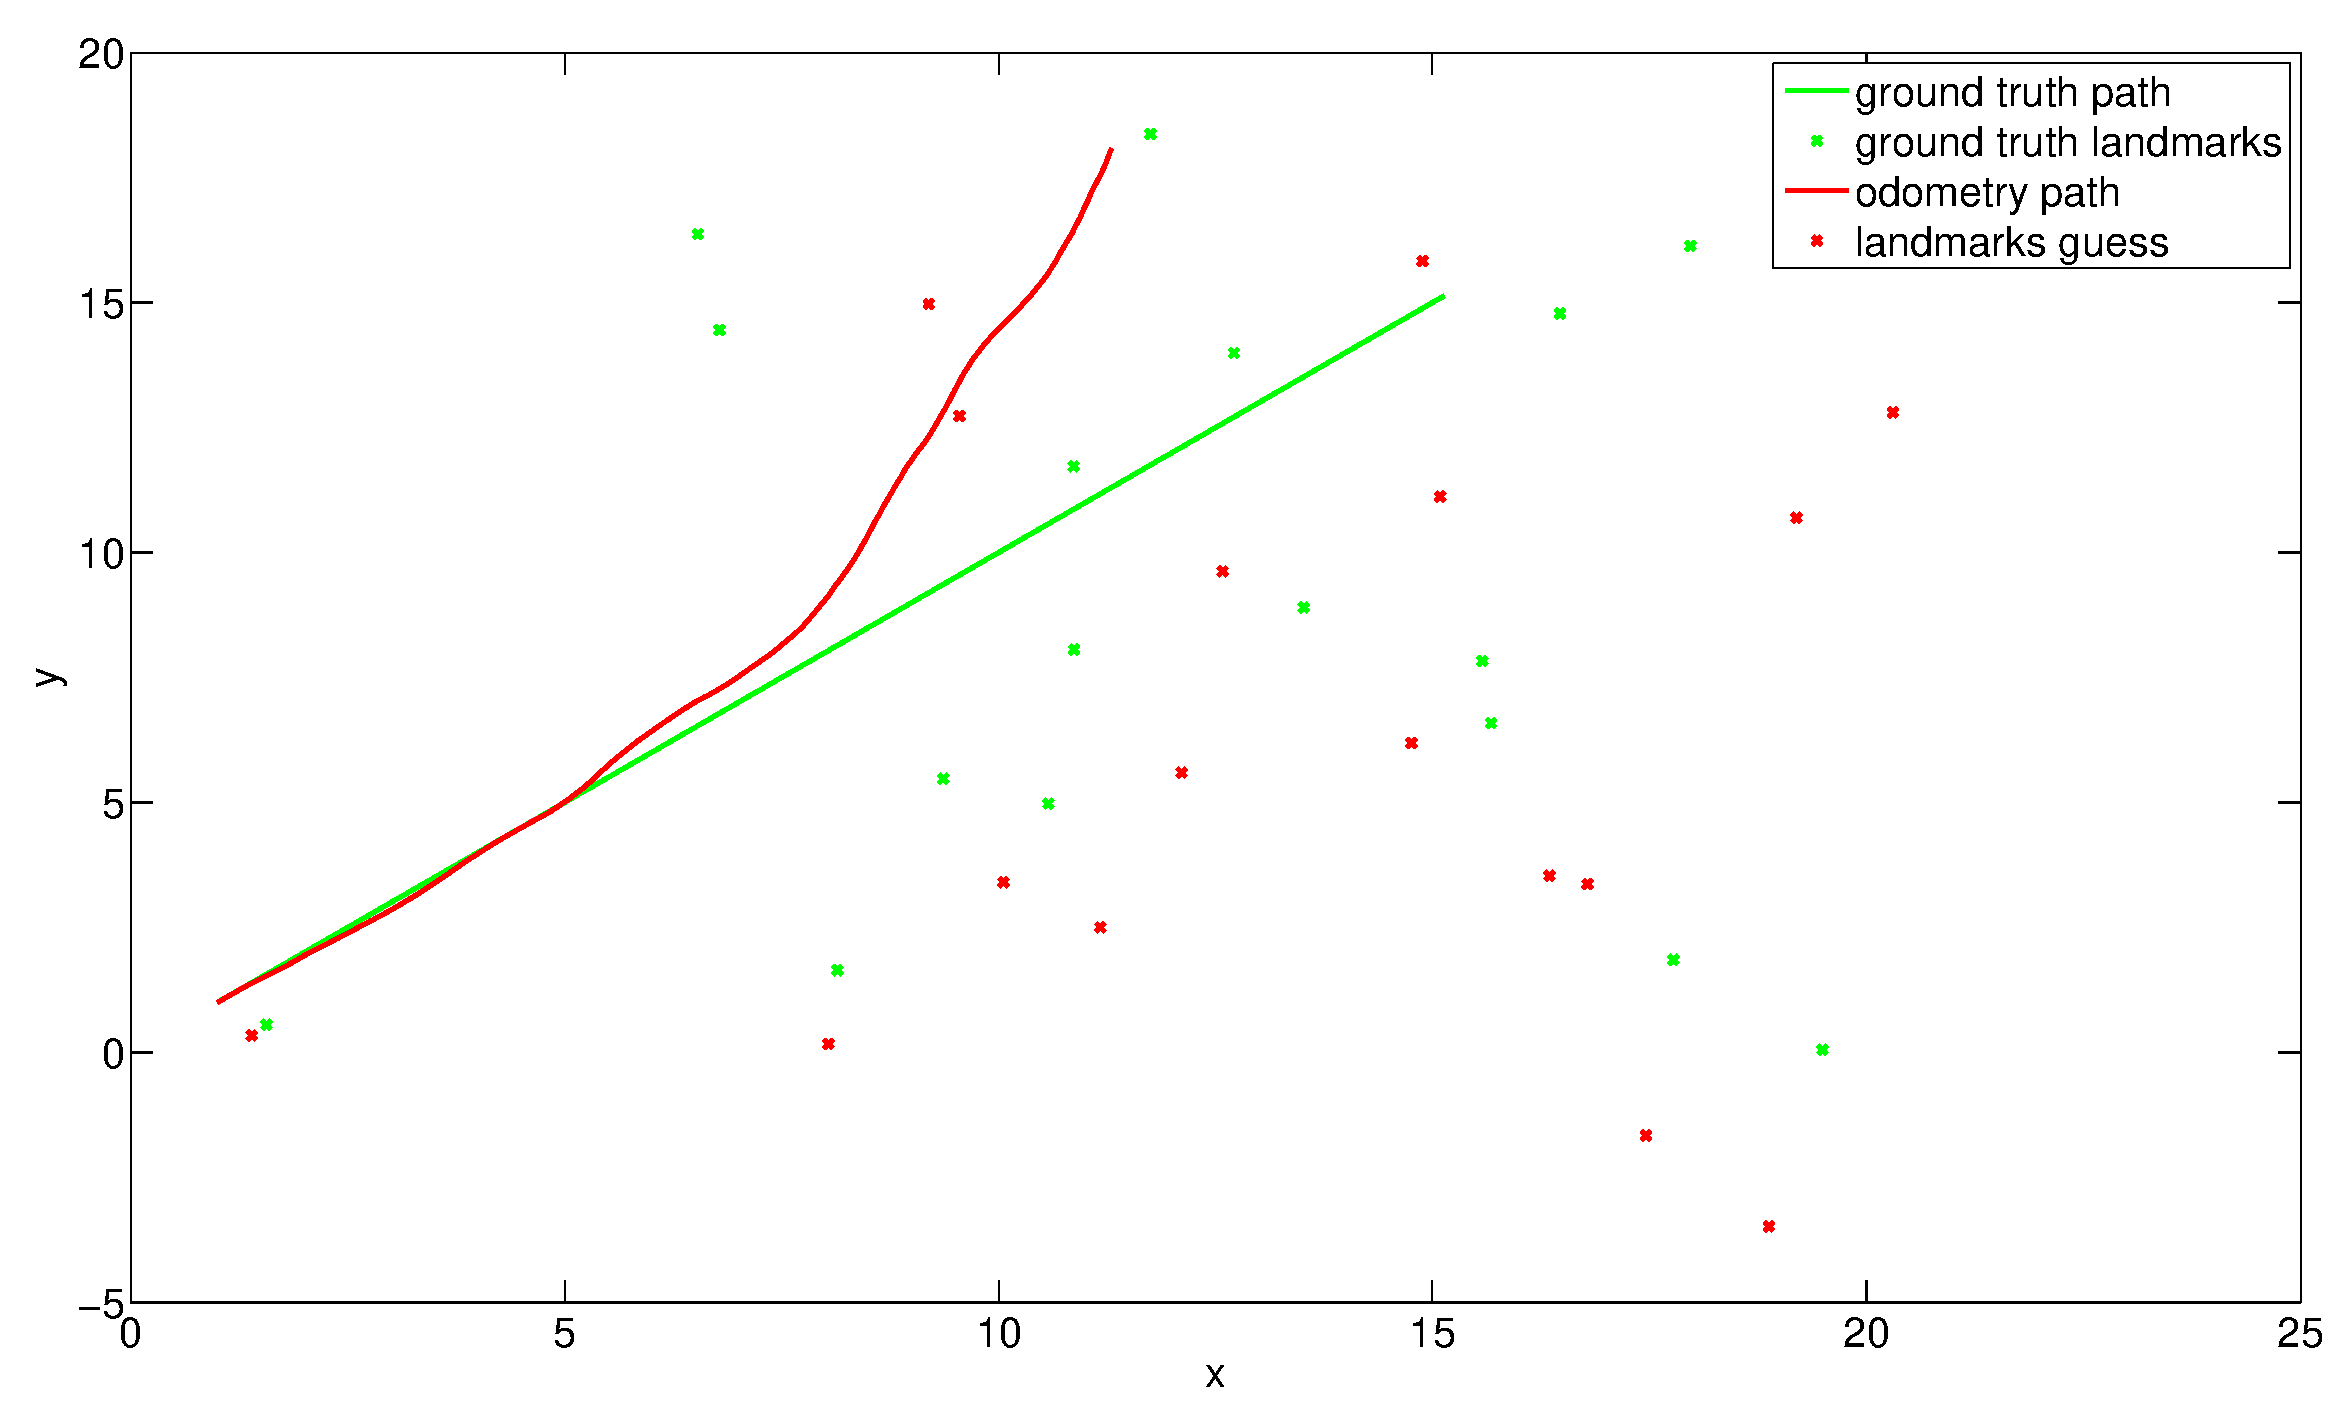
\includegraphics[width=\columnwidth]{fig/straight-path.eps}
\caption{Straight path example (best viewed in color). The green line
  represents the ground truth path, the red line the integrated odometry path,
  the green crosses the ground truth landmark positions, and the red crosses the
  guessed landmark positions from measurements.}
\label{fig:straight-path}
\end{figure}

\begin{figure}[t]
\centering
\begin{minipage}{.492\columnwidth}
  \centering
  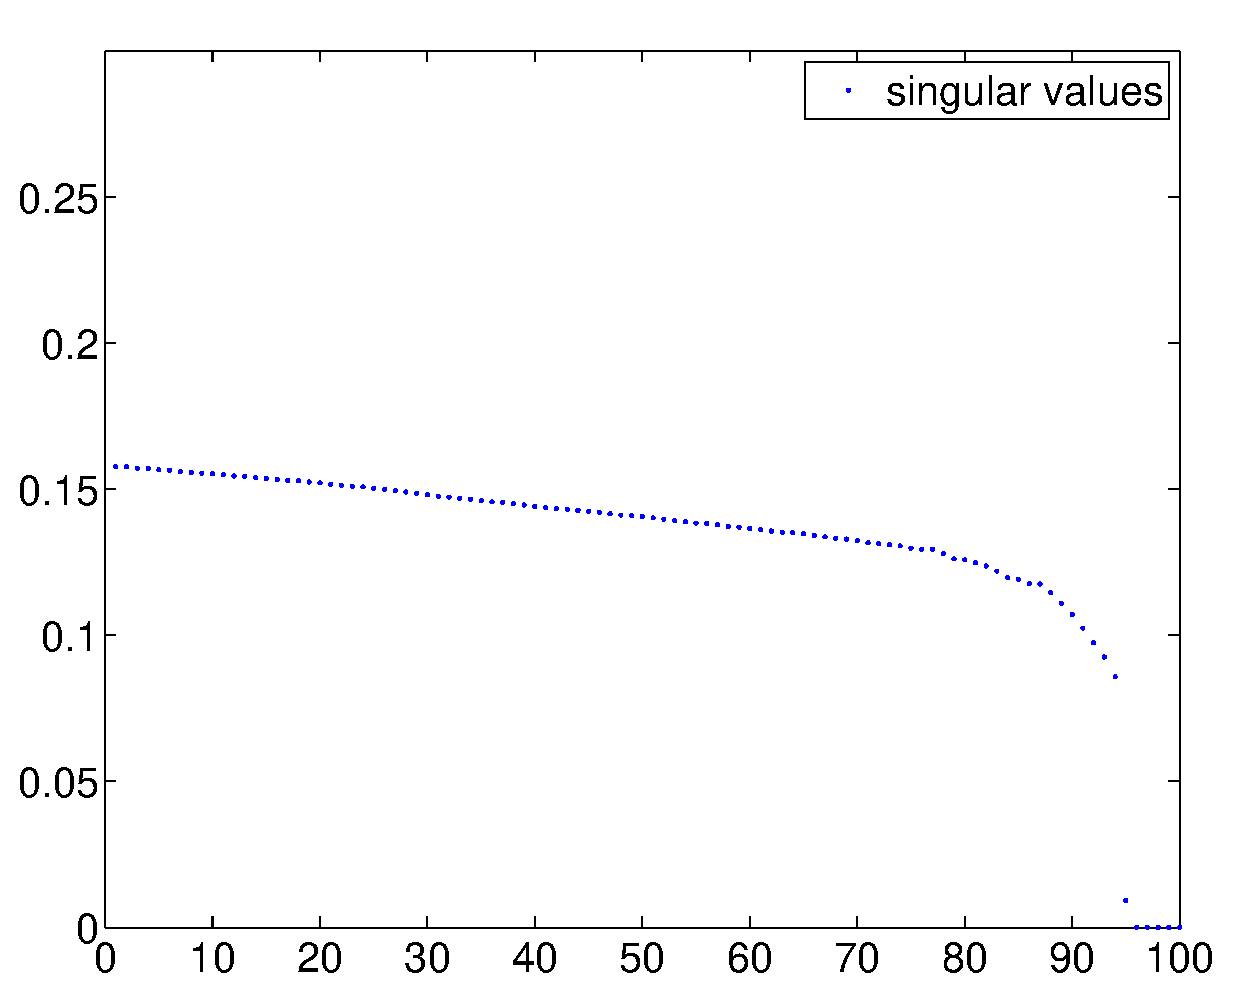
\includegraphics[width=\columnwidth]
    {fig/straight-path-noisefree-svd-scaled.eps}
\end{minipage}
\begin{minipage}{.492\columnwidth}
  \centering
  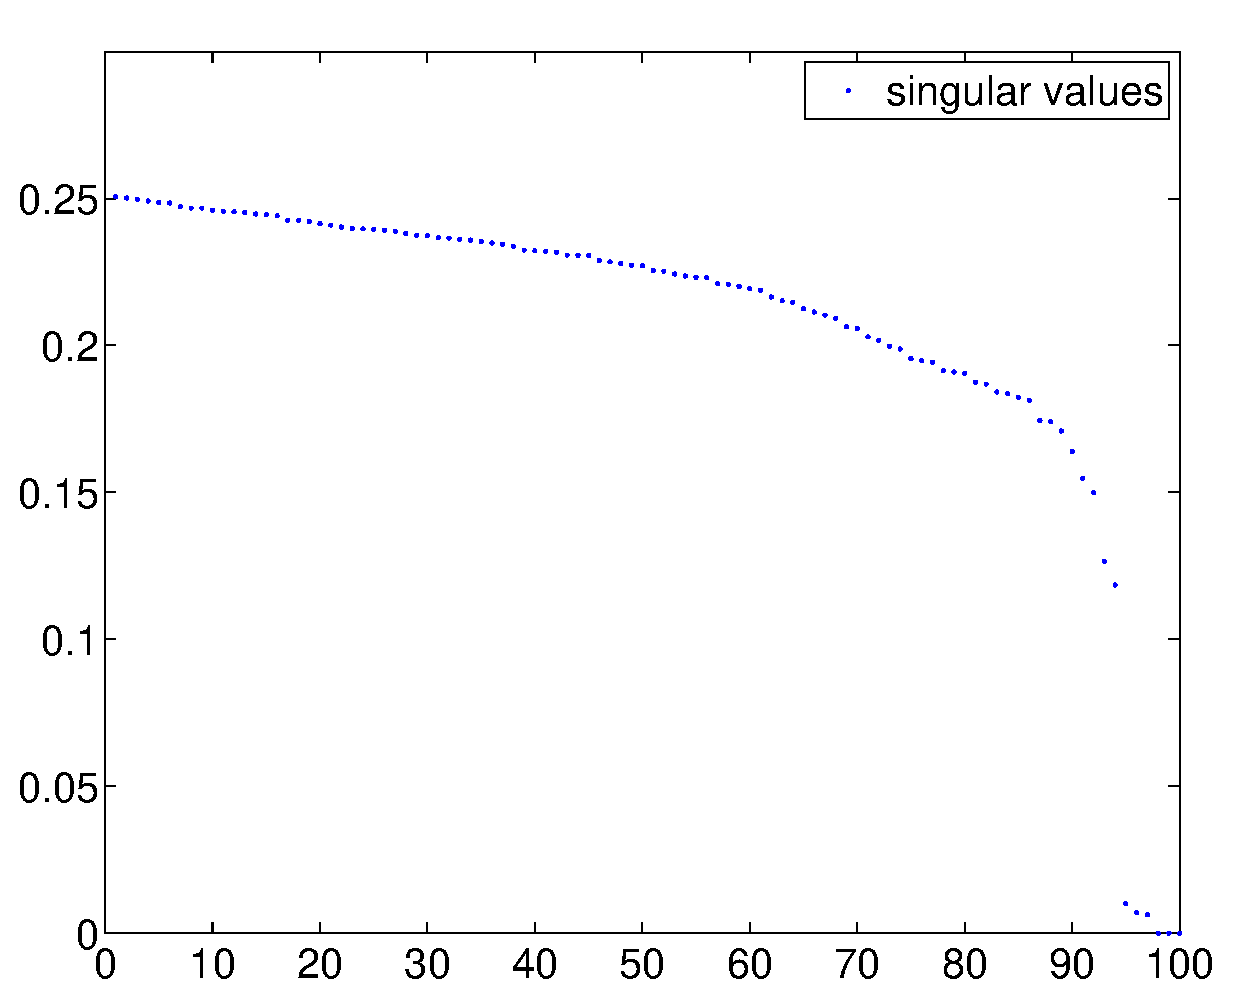
\includegraphics[width=\columnwidth]
    {fig/straight-path-svd-scaled.eps}
\end{minipage}
\begin{minipage}{.492\columnwidth}
  \centering
  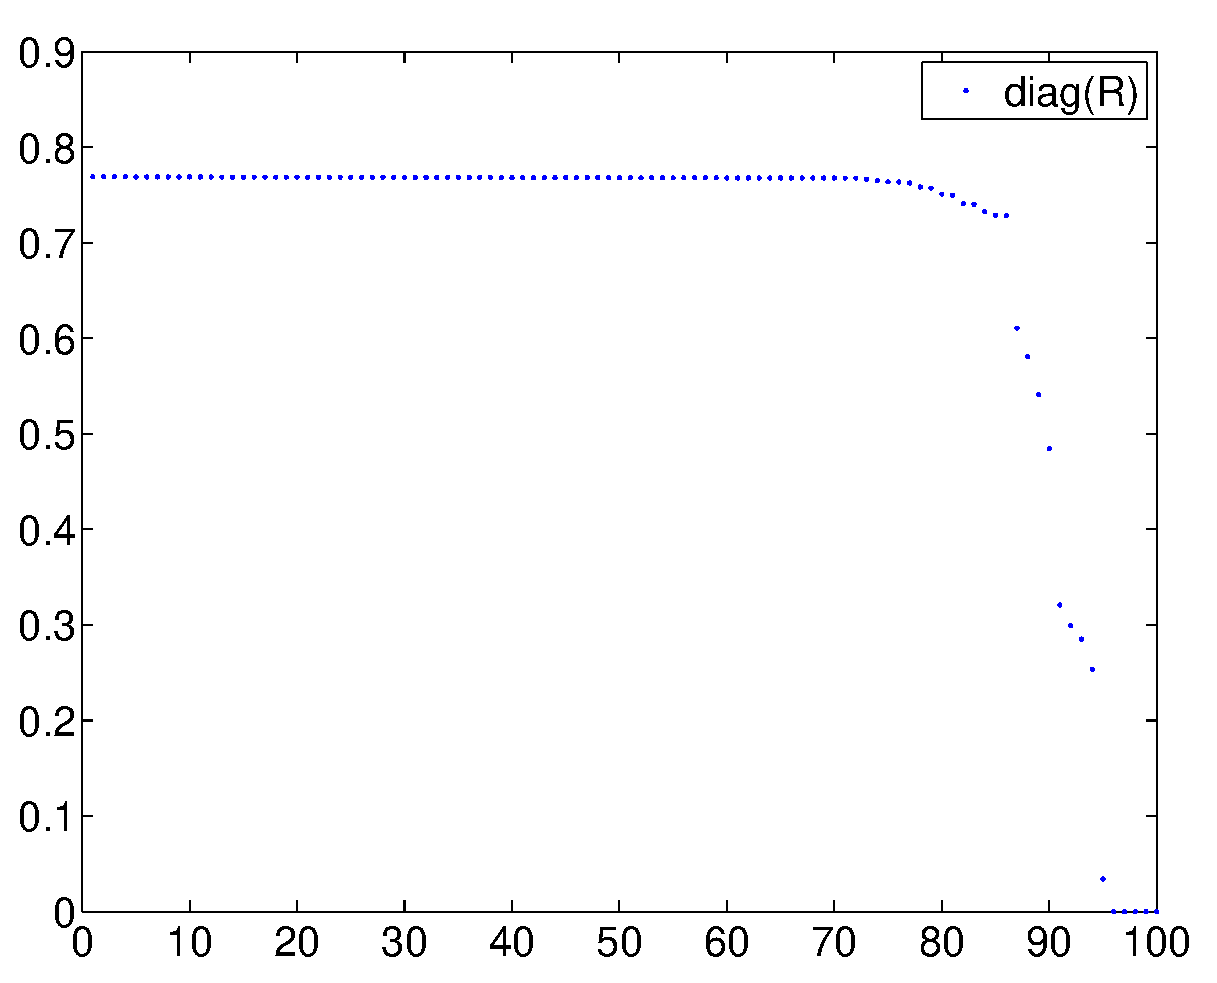
\includegraphics[width=\columnwidth]
    {fig/straight-path-noisefree-spqr-scaled.eps}
\end{minipage}
\begin{minipage}{.492\columnwidth}
  \centering
  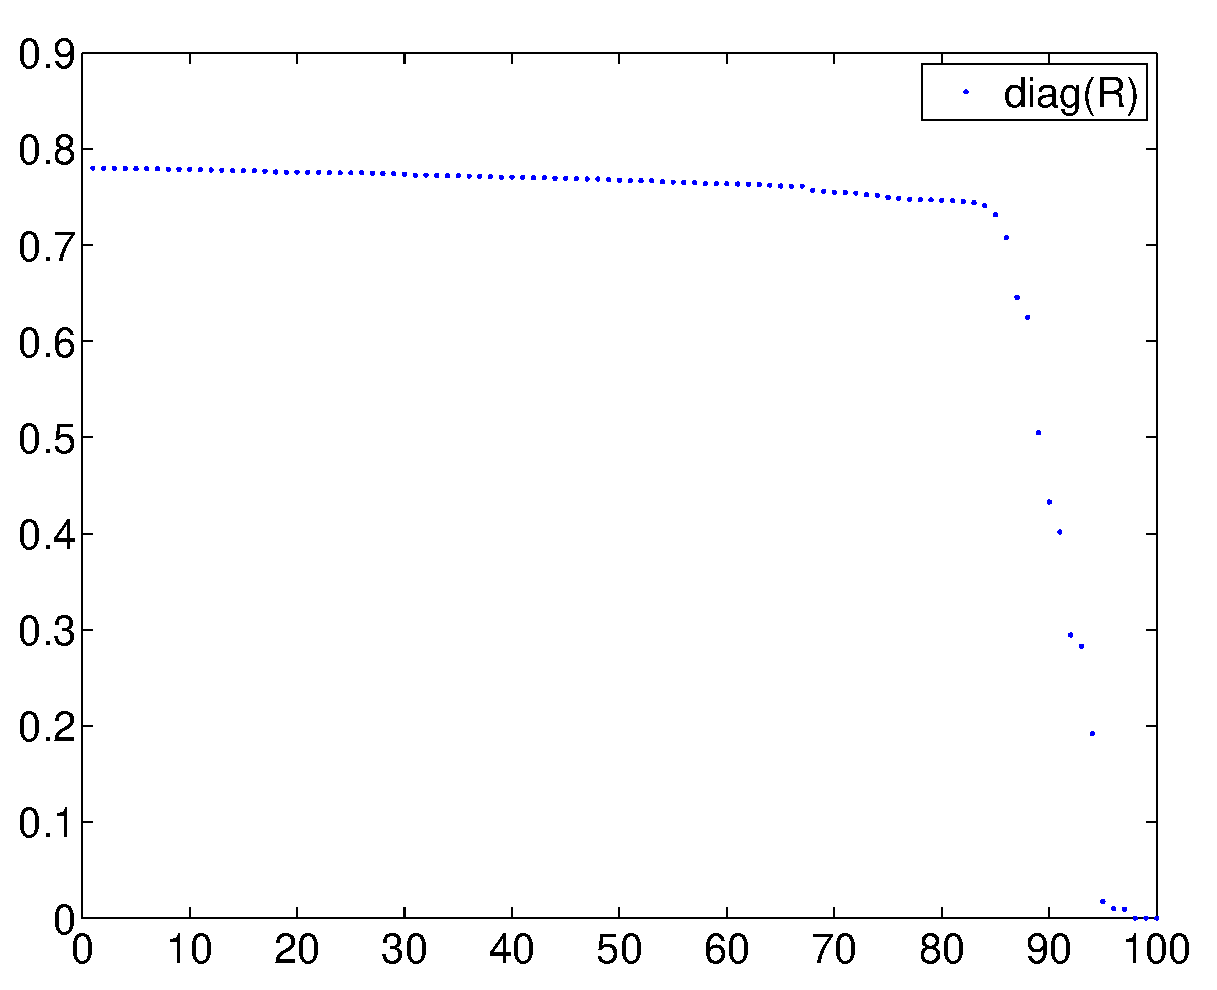
\includegraphics[width=\columnwidth]
    {fig/straight-path-spqr-scaled.eps}
\end{minipage}
\caption{Straight path example analysis. The first column shows the singular
  values and the diagonal elements of the $\mathbf{R}$ matrix from the QR
  decomposition in the noise-free case, and the second column in the noisy
  case. Only the 100 lower values from the scaled system
  \eqref{eqn:scaled_system} are plotted for visualization purpose.}
\label{fig:straight-path-analysis}
\end{figure}

For this first example, Fig.~\ref{fig:straight-path-time} shows the mean
computation time for some dataset sizes over 100 repetitions for one iteration
of the Gauss-Newton algorithm using SVD and sparse QR decomposition on a
quad-core desktop machine. It usually takes less than 10 iterations for the
optimization to converge. Nevertheless, the SVD method rapidly becomes
prohibitive due to the polynomial computation time.

\begin{figure}[t]
\centering
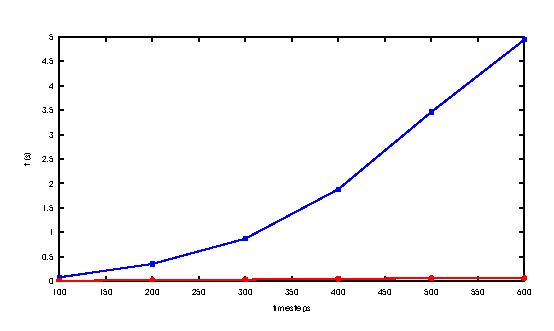
\includegraphics[width=\columnwidth]{fig/straight-path-time.eps}
\caption{Mean computation time over 100 repetitions for one step of
  optimization using SVD (polynomial time) and sparse QR (linear time)
  decomposition.}
\label{fig:straight-path-time}
\end{figure}

To conclude this section on simulated data, we will analyze the performance of
different algorithms, namely an Extended Kalman Filter (EKF) similar
to~\cite{martinelli06automatic}, a standard batch nonlinear least squares
method without regularization~\cite{kuemmerle11simultaneous}, and our TQR-MI
approach, on the straight path scenario and on a well-behaved path with turns.
We have repeated the experiments 100 times with the same initial conditions.

\subsection{Real-world Data}

In order to validate our method on real-world data, we have used the ``Lost in
the Woods Dataset'' provided with the courtesy of Tim
Barfoot~\cite{tong12gaussian}. This dataset contains approximately $20$ minutes
of a robot driving amongst a forest of tubes which serve as landmarks. The
ground truth comes from a motion capture system that tracks robot motion and
tube locations. For the calibration parameters, we have only access to
$\delta_x=0.219$ [m] that was roughly measured with a tape. We assume the others
are implicitly set to $0$ ($\delta_y=0$ [m] and $\psi=0$ [rad]).
Fig.~\ref{fig:dataset2-path-result} displays the qualitative result of our
algorithm. Using only $10\%$ of the measurements, we could recover accurate
landmark positions, robot poses, and calibration parameters. For visualization,
estimated landmarks and poses have
been aligned to the ground truth using the algorithm
from~\cite{fiore01efficient}.

\begin{figure}[t]
\centering
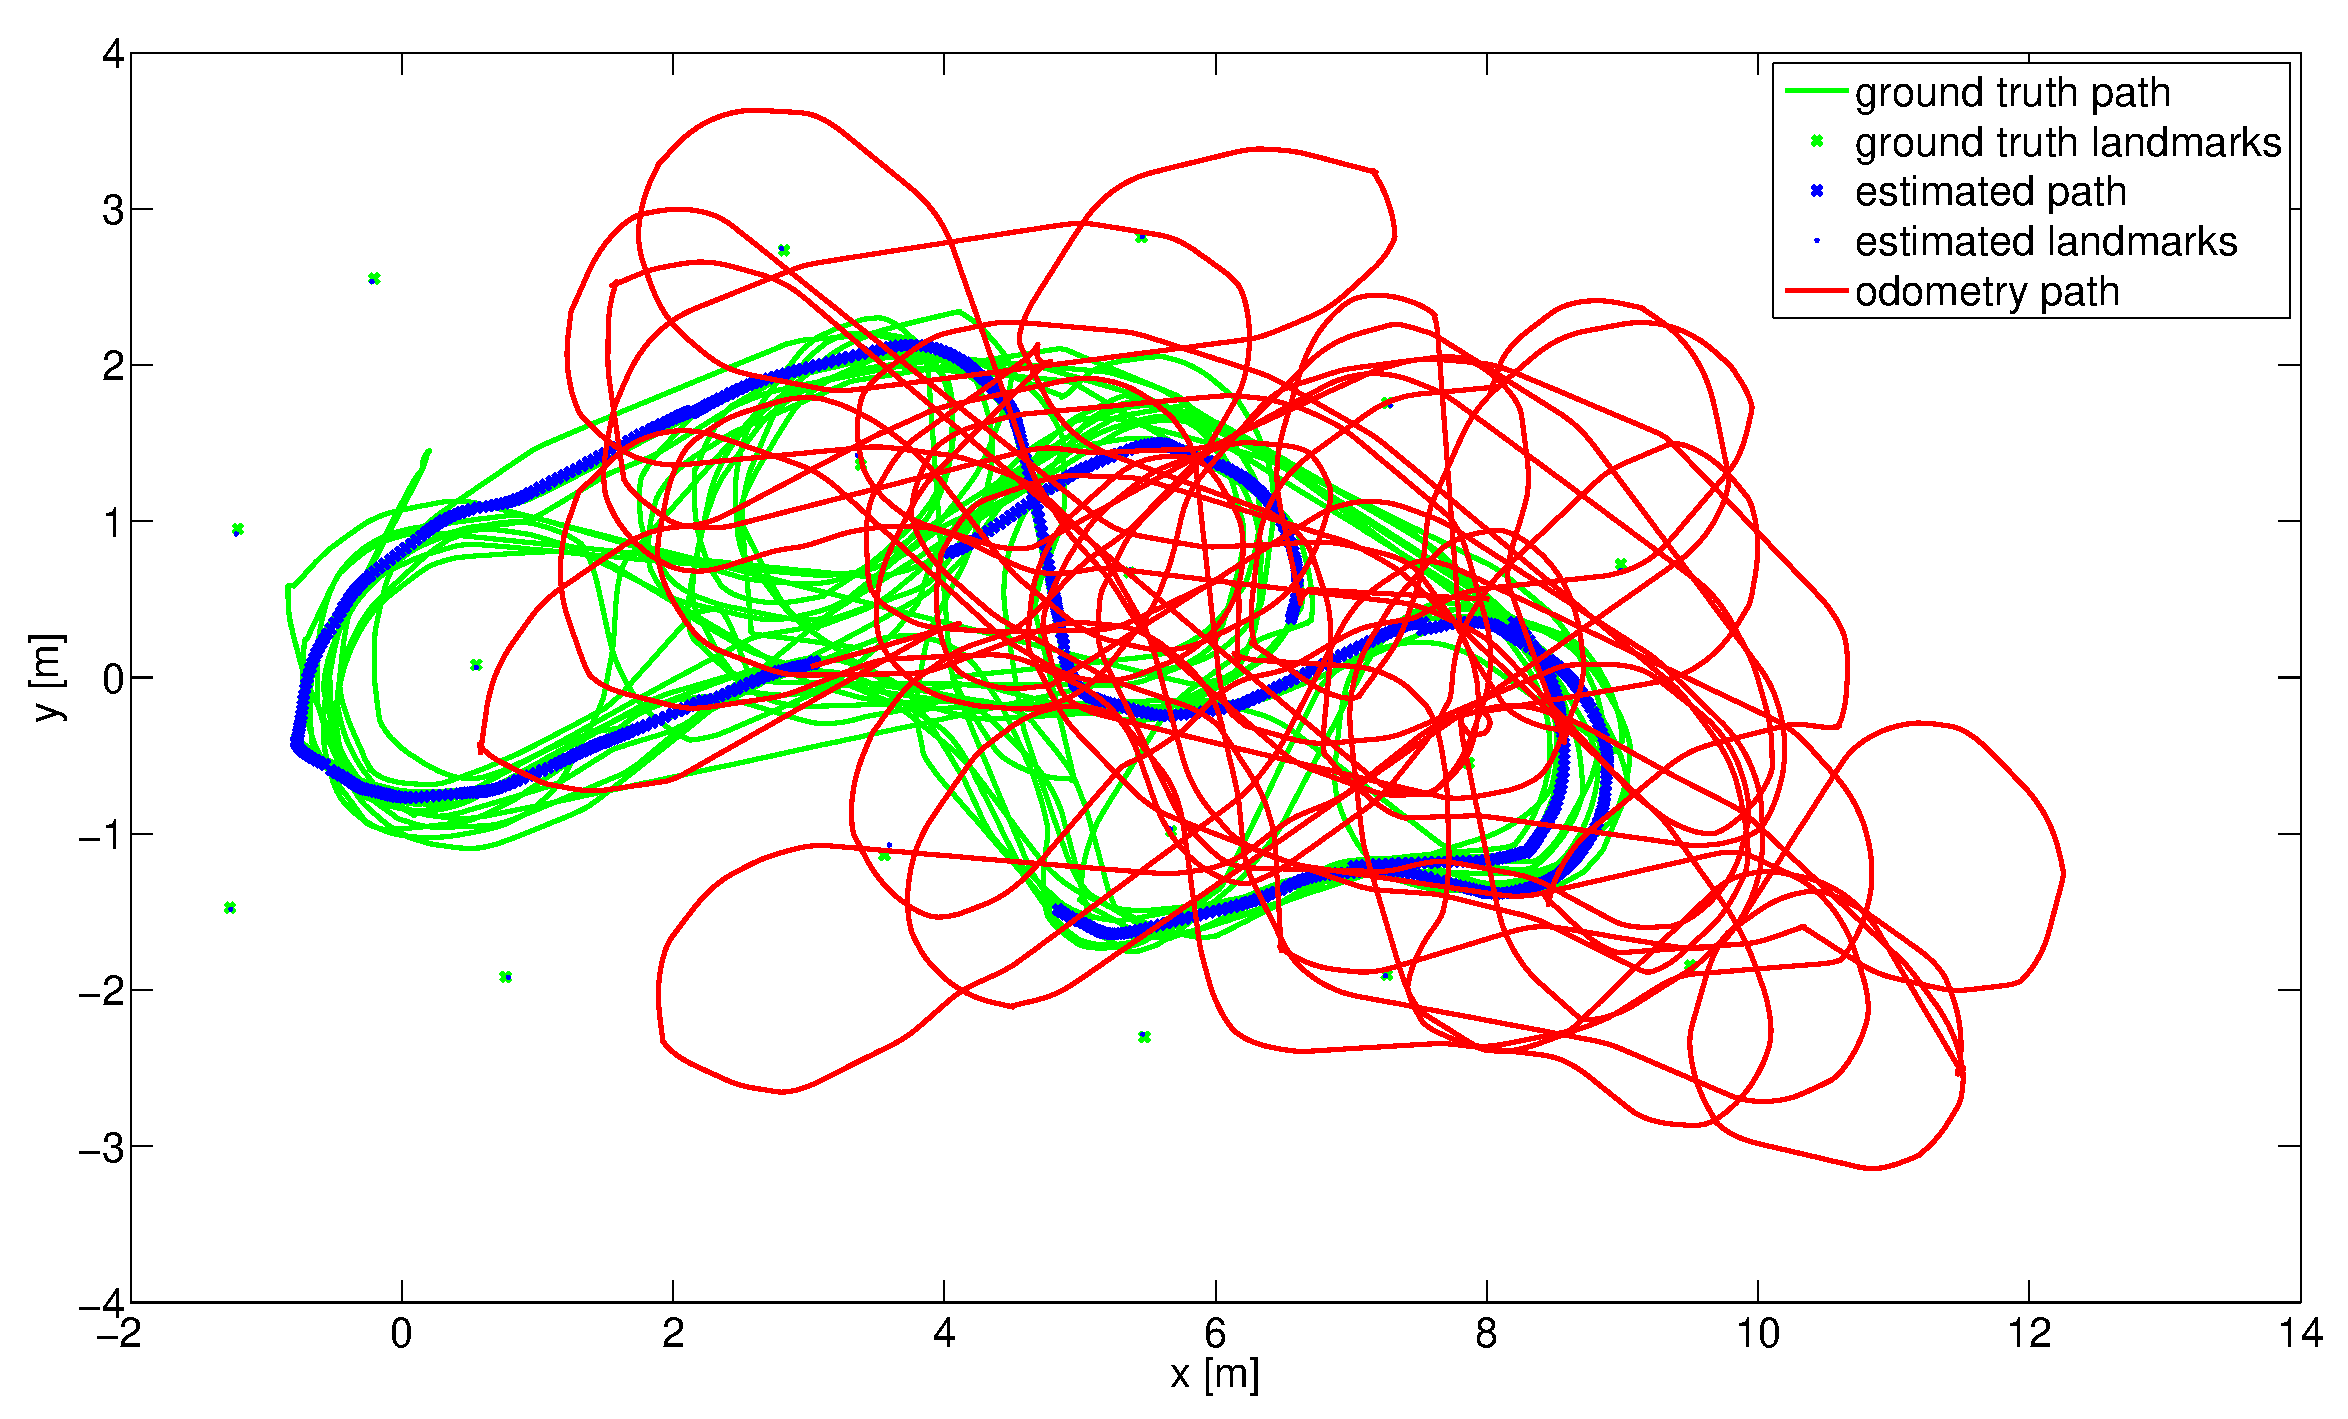
\includegraphics[width=\columnwidth]{fig/dataset2-path-result.eps}
\caption{Application of our algorithm on the ``Lost in the Woods dataset''
  (best viewed in color). The
  green line represents the ground truth path, the red line the integrated
  odometry path, the green crosses the ground truth landmark positions, the blue
  points the estimated landmark positions, and the blue crosses the estimated
  robot poses. Our MI selection scheme picks only $10\%$ of the measurements
  for the optimization.}
\label{fig:dataset2-path-result}
\end{figure}

Since the ground truth calibration parameters are inaccurate,
Tab.~\ref{tab:dataset2-comp} compares our method against a standard
least squares (LS) estimator that exploits all the measurements. Our TQR-MI
algorithm performs the optimization with $K=1209$ out of $12609$ timesteps.
Although the calibration parameters are the same magnitude, the higher variances
stem from the fewer number of considered measurements.

\begin{table}[!t]
\renewcommand{\arraystretch}{1.3}
\caption{Comparison of a standard least squares estimator and our
  method on the ``Lost in the Woods dataset''.}
\label{tab:dataset2-comp}
\centering
\begin{tabular}{c||c||c}
\hline
& \bfseries LS & \bfseries TQR-MI\\
\hline\hline
$\hat{\delta}_x$ [m] & $0.2363$ & $0.2344$\\
\hline
$\hat{\delta}_y$ [m]& $0.0034$ & $0.0087$\\
\hline
$\hat{\psi}$ [rad] & $0.0810$ & $0.0754$\\
\hline
$\hat{\Sigma}_{\delta_x}$ [$\text{m}^2$] & $0.0892\times 10^{-5}$ &
  $0.1903\times 10^{-4}$\\
\hline
$\hat{\Sigma}_{\delta_y}$ [$\text{m}^2$] & $0.39\times 10^{-5}$ &
  $0.7243\times 10^{-4}$\\
\hline
$\hat{\Sigma}_{\psi}$ [$\text{rad}^2$] & $0.0254\times 10^{-5}$ &
  $0.0582\times 10^{-4}$\\
\hline
$K$ & $12609$ & $1209$\\
\hline
\end{tabular}
\end{table}


\section{Conclusion\label{sec:conc}}
In this paper, we have presented a novel approach to the automatic calibration
of mobile robot sensors. We have included the calibration parameters in a SLAM
formulation and computed an MAP estimator using a Gauss-Newton algorithm. To
cope with unobservability, we have employed truncated QR decomposition as a
regularization method. For long-term and online operations, we have devised
a mutual information selection scheme that solely captures informative
measurements relevant to the calibration. Our algorithm has been thorougly
tested and validated through extensive simulated and real-world experiments on
a 2D robot equipped with a laser range finder.

In the near future, we will consider the self calibration of multiple sensors
(cameras, 3D/2D LRF, GPS/INS system) mounted on an autonomous car. From a
research point of view, we would like to further automate the selection of the
free parameters. Lastly, we want to detect...\todo{To be discussed}.


\section*{Acknowledgment}
This work has partly been supported by the EC under FP7-269916-V-Charge.

\bibliographystyle{sty/IEEEtran}
\bibliography{bib/bibliography}

\end{document}
